\chapter{Continuous Integration}
\section{Einleitung}\label{sec:einleitung}
Während des Verlaufes der Diplomarbeit wurde es notwendig unsere Applikation auf einen Server der HTL Leonding zu deployen. Genauer gesagt musste das JavaEE Backen auf einen Application Sever deployed werden. Um jedoch nicht immer per Hand bei der kleinsten Änderung das Projekt neu zu compilieren und dann manuell zu deployen, wurde entschieden diesen Prozess mithilfe von continuous Integration zu vereinfachen.

\section{Was ist CI?}\label{sec:cierklärung}
Continuous Integration (CI) ist ein Teil der modernen Software Entwicklung. CI stellt den Prozess dar, der das Bauen und Testen einer Anwendung abbildet. Mit Hilfe von CI lassen sich Fehler schneller finden und beheben. Die Idee der kontinuierlichen Integration ist es, dass die Entwickler frühzeitig und regelmäßig Änderungen in das Versionsmanagement einchecken. Diese Änderungen sollten funktionsfähig sein, sodass die gesamte Applikation auf Integrationsprobleme geprüft werden kann.

Es ist somit die Verfügbarkeit einer lauffähigen Version gegeben, die dann zum Beispiel für anderweitige Testzwecke oder Vertriebszwecke genutzt werden kann. Eine typische Anwendung sind sogenannte Nightly Builds, bei denen zu einer vorgegebenen Uhrzeit der aktuelle Programmcode übersetzt wird und dabei Tests mit der erstellten Software automatisch ausgeführt werden. Bei gefundenen Problemen kann ein Entwickler dann zum Beispiel direkt per Mail über das gefundene Problem informiert werden.

\section{Wieso CI?}\label{sec:whyci}
Continuous Integration hat das Ziel, die Qualität der Software über permanente Integration ihrer einzelnen Bestandteile zu steigern. Statt die Software nur in sehr großen Zeitabständen kurz vor der Auslieferung zu erstellen, wird sie in kleinen Zyklen immer wieder erstellt und getestet. Es ist auch ein Zeitgewinn vorhanden da nicht nach jedem Zyklus die Software per Hand sondern auf Knopfdruck ausgeliefert und getestet wird.

\section{Wie kann CI realisiert werden?}\label{sec:whyci}
Folgende Tools kamen für diese Herausforderung in Frage:

\textbf{Bambo}
Bamboo ist ein continuous integration server von Atlassian, den Entwicklern von JIRA, Confluence and Crowd. 

\textbf{Travis CI}

Travis CI ist ein open-source gehosteter, continuous integration Service, der sehr stark in  GitHub integriert ist.

\textbf{Jenkins}

Jenkins ist ein webbasiertes Open Source Continous Integration System. Es ist in Java geschrieben und plattformunabhängig. Die Basis von Jenkins unterstützt zahlreiche Werkzeuge darunter SVN, Ant, Maven sowie JUnit. Durch die Community können weitere Funktionen mithilfe von Plug-Ins hinzugefügt werden. Somit lässt sich Jenkins für jedes Projekt individuell anpassen. Auch für Projekte mit anderen Sprachen/Technologien wie zum Beispiel PHP, Ruby oder .NET ist Jenkins geeignet. Testwerkzeuge lassen sich mittels Plug-Ins über die intuitive Benutzeroberfläche integrieren. Builds können durch verschiedene Auslöser gestartet werden: zum Beispiel Änderung des CVS oder Zeitplan (zum Beispiel Nightly Builds). Nightly Builds sind besonders bei Open Source Projekten zu finden und bedeutet, dass die Applikation nachts gebaut und getestet wird.

Aufgrund der hohen Anpassungsmöglichkeit, der großen Community und der sehr genauen Dokumentation, wird Jenkins als Tool für die Continous Integration ausgewählt.

\section{Jenkins installieren}
\label{sec:jenkinsinstallation}
Auf unsere Ubuntu 16.04 Server wurde Jenkins mittels Console installiert und es musste das Jenkins Apt-Repository dem Server apt-repository mit folgendem Befehl: "wget -q -O - https://pkg.jenkins.io/debian/jenkins-ci.org.key | sudo apt-key add -" und 
"sudo sh -c 'echo deb http://pkg.jenkins.io/debian-stable binary/ > /etc/apt/sources.list.d/jenkins.list'" hinzugefügt werden.

Bevor Jenkins installiert wird, wird das Ubuntu Apt-Repository aktualisiert mit ''sudo apt-get update" und dann kann Jenkins installiert werden mit ''sudo apt-get install jenkins''.

Nachdem der Installer fertig ist, wird wie in der Abbildung \ref{img:consoleoutput} ein initialAdminPassword angezeigt. Dieses wird benötigt um die weiteren Schritte von der Jenkins Installation zu autorisieren.

\begin{figure}[h]
\centering
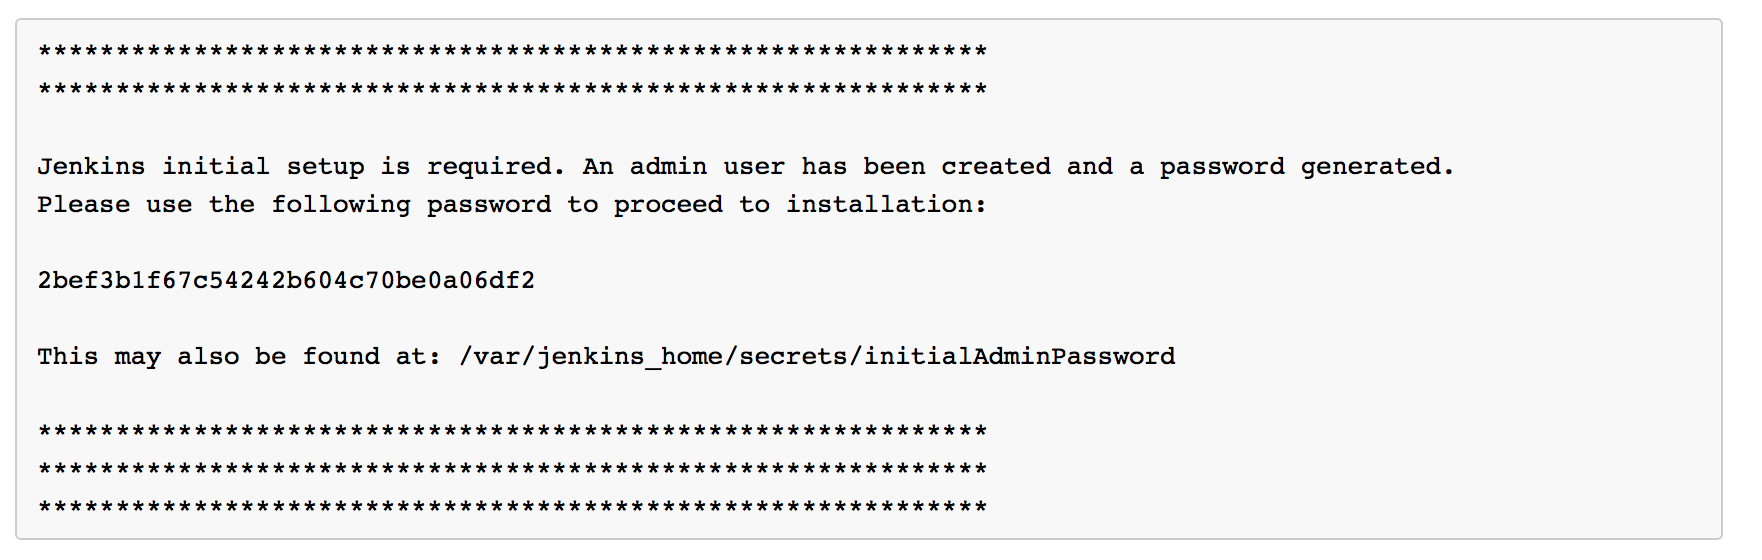
\includegraphics[width=1\textwidth]{images/09_CI/consoleOutput.png}
\caption{Konsolen Ausgabe - Jenkins}
\label{img:consoleoutput}
\end{figure}

Nachdem das initialAdminPassword ausgegeben wurde, kann Jenkins unter der ServerUrl  und dem Standard Port 8080 erreicht werden. 

\begin{figure}[h]
\centering
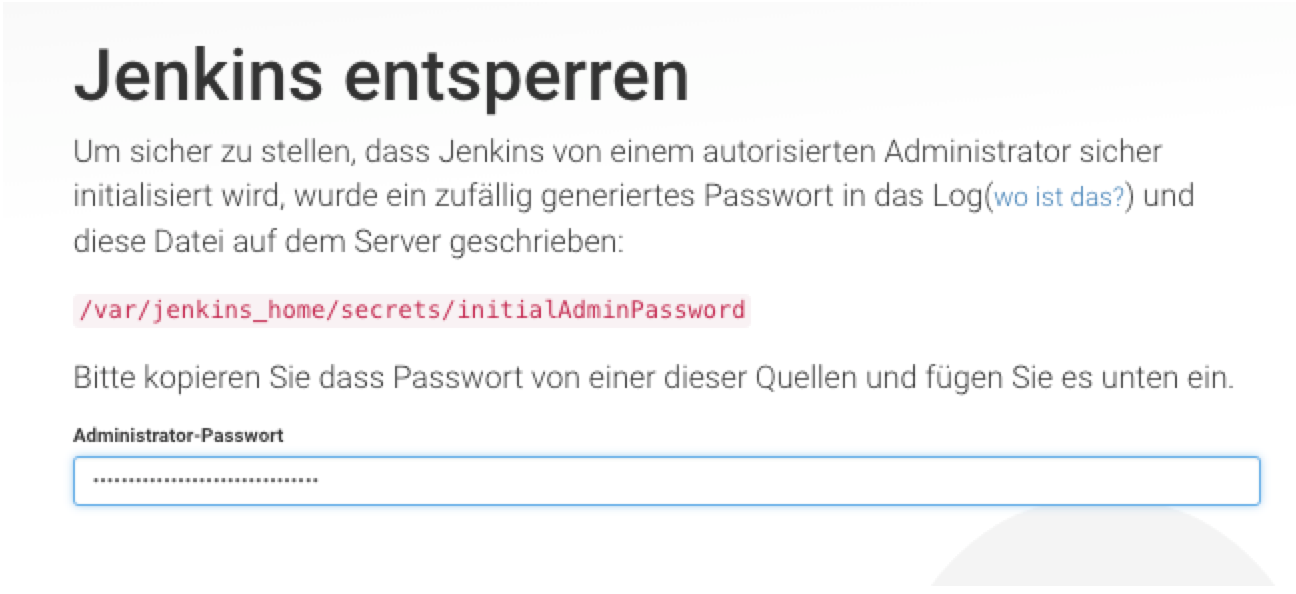
\includegraphics[width=1\textwidth]{images/09_CI/initial.png}
\caption{Anmelden - Jenkins}
\label{img:login}
\end{figure}

Wie in \ref{img:login} muss das Passwort jetzt eingegeben werden um die Installation fortzusetzen. In den nächsten Ansichten muss ein Admin User angelegt werden und die benötigten Plug-Ins für den Jenkins ausgewählt werden. Hier reichen die Standard Plug-Ins völlig aus.

Jetzt kann Jenkins verwendet werden.

\section{Jenkins CI konfigurieren}
\label{sec:jenkinsconfiguration}
Um jetzt eine JavaEE Anwendung mithilfe vom Jenkins auf einen Wildfly Application Server zu deployen, müssen vorher noch die Enviroment Variablen, JDK's, Maven und der Application Server auf dem Server konfiguriert werden. Die Enviroment Variablen, JDK's und Maven werden vom Jenkins eingerichtet. Dann muss nur in den Einstellungen die jeweilige Version konfiguriert werden. Zusätzlich es muss ein Oracle Login hinterlegt werden, damit sich Jenkins das Java JDK herunterladen kann und das GitHub Konto in welchem sich die Repositories befinden. Jedoch muss der Wildfly manuell heruntergeladen und konfiguriert werden.

Nachdem alle Entwicklungskits installiert sind, kann nun eine Pipeline im Jenkins eingerichtet werden. Dabei wird im Jenkins ein FreeStyle Softwareprojekt erstellt. Des Weiteren muss das Repository und der Branch angegeben werden. Damit Builds von außerhalb von Jenkins ausgeführt werden können, muss die Option ''Builds von außerhalb starten (z.B. skriptgesteuert)'', aktiviert und ein Authentifizierungstoken eingetragen werden. Das Builden ist das Erstellen einer neuen Version von einem Programm. Damit nach jedem ''Commit'' ein neuer Build gestartet wird muss die Option ''GitHub hook trigger for GITScm polling'' ebenfalls aktiviert werden. Bei der Funktion ''Build'' muss der Pfad zur POM des Servers angegeben und welches Maven-Goal ausgeführt werden soll, also 'install'. Mit dem ''install'' Maven-Goal werden direkt beim Build die Unit Tests ausgeführt.

Nachdem ''Builden'' muss die fertige ''.war'' File auf dem Wildfly Application Server deployed werden. Dieses Skript wird nach dem erfolgreichem Build vom Jenkins ausgeführt. Das Skript verwendet die Jboss-CLI. Dabei muss man sich auf den Application Server verbinden und den Befehl ''deploy'' ausführen, mit dem Pfad zur ''.war'' File. (siehe Code Beispiel \ref{lst:deploy}) 

\begin{lstlisting}[language=bash,caption={Deploy war-File},label={lst:deploy}]
bash /home/vwall/wildfly-10.1.0.Final/bin/jboss-cli.sh --controller=vm59.htl-leonding.ac.at:9990 --connect -u=USER -p=PASSWORD --command="deploy --force /var/lib/jenkins/workspace/HomeDsSystems_Backend/
	HomeDsBackend/target/homeds.war"
\end{lstlisting}


